%%% 
%% Project Management :: Planning 
%%% 
\section{Planning}
\label{sec:planning}

This section contains the project plans which have been developed in Microsoft
Project 2010. There are three sub sections which define the initial, interim and end progress of the project. \citet{planning05} refers to software engineering as two domains.

\begin{enumerate}
\item Student Systems - Programs that people build to illustrate something or for hobby.
\item Industrial Strength Software - Software that can lead to significant direct or indirect loss.
\end{enumerate}

A software project that is planned throughly is a more successful project than a project that is developed through extreme programming. The Cryptic Crossword project initially started through the Waterfall life cycle model and gradually grew to become an Iterative model. Therefore the project plans had to be updated constantly to reflect the change in which the project was being undertaken. Although the overall project is developed in the Waterfall model due to the time constraints applied by University deadlines the project consists of an iterative development outside of the deliverables which are to be produced for academic purposes. 

\newpage 
\begin{landscape}


\subsection{Timeline}

\begin{figure}[H]
  \centering
  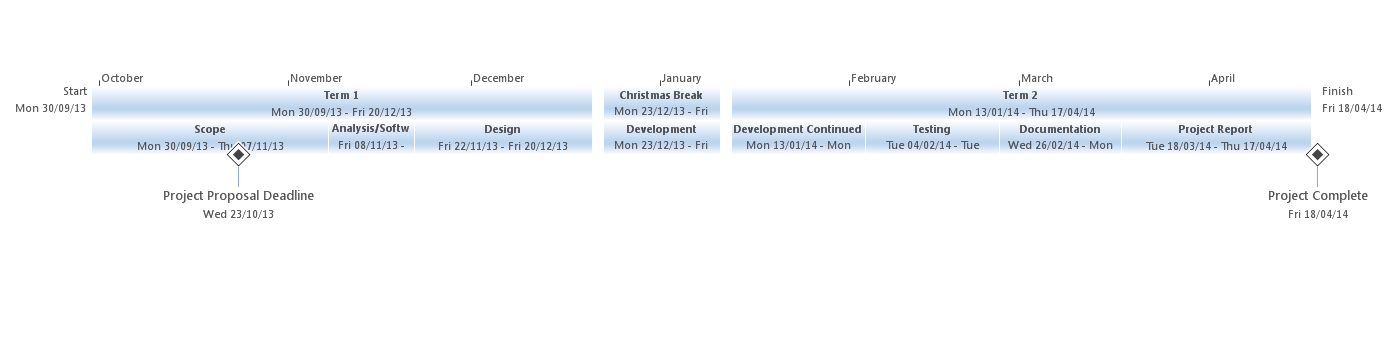
\includegraphics[width=\linewidth]{images/timeline1.png}
  \caption{Project Timeline on the 21st October 2013}
  \label{fig:timeline1}
\end{figure}

Figure ~\ref{fig:timeline1} shows the initial timescale that was drawn up while planning the project. This was produced to show the major deliverables and their dates. In the next section the Gantt Chart that was produced with all the initial tasks to be completed are shown. 

\newpage 
\subsection{Initial Gantt Chart}

\begin{figure}[H]
  \centering
  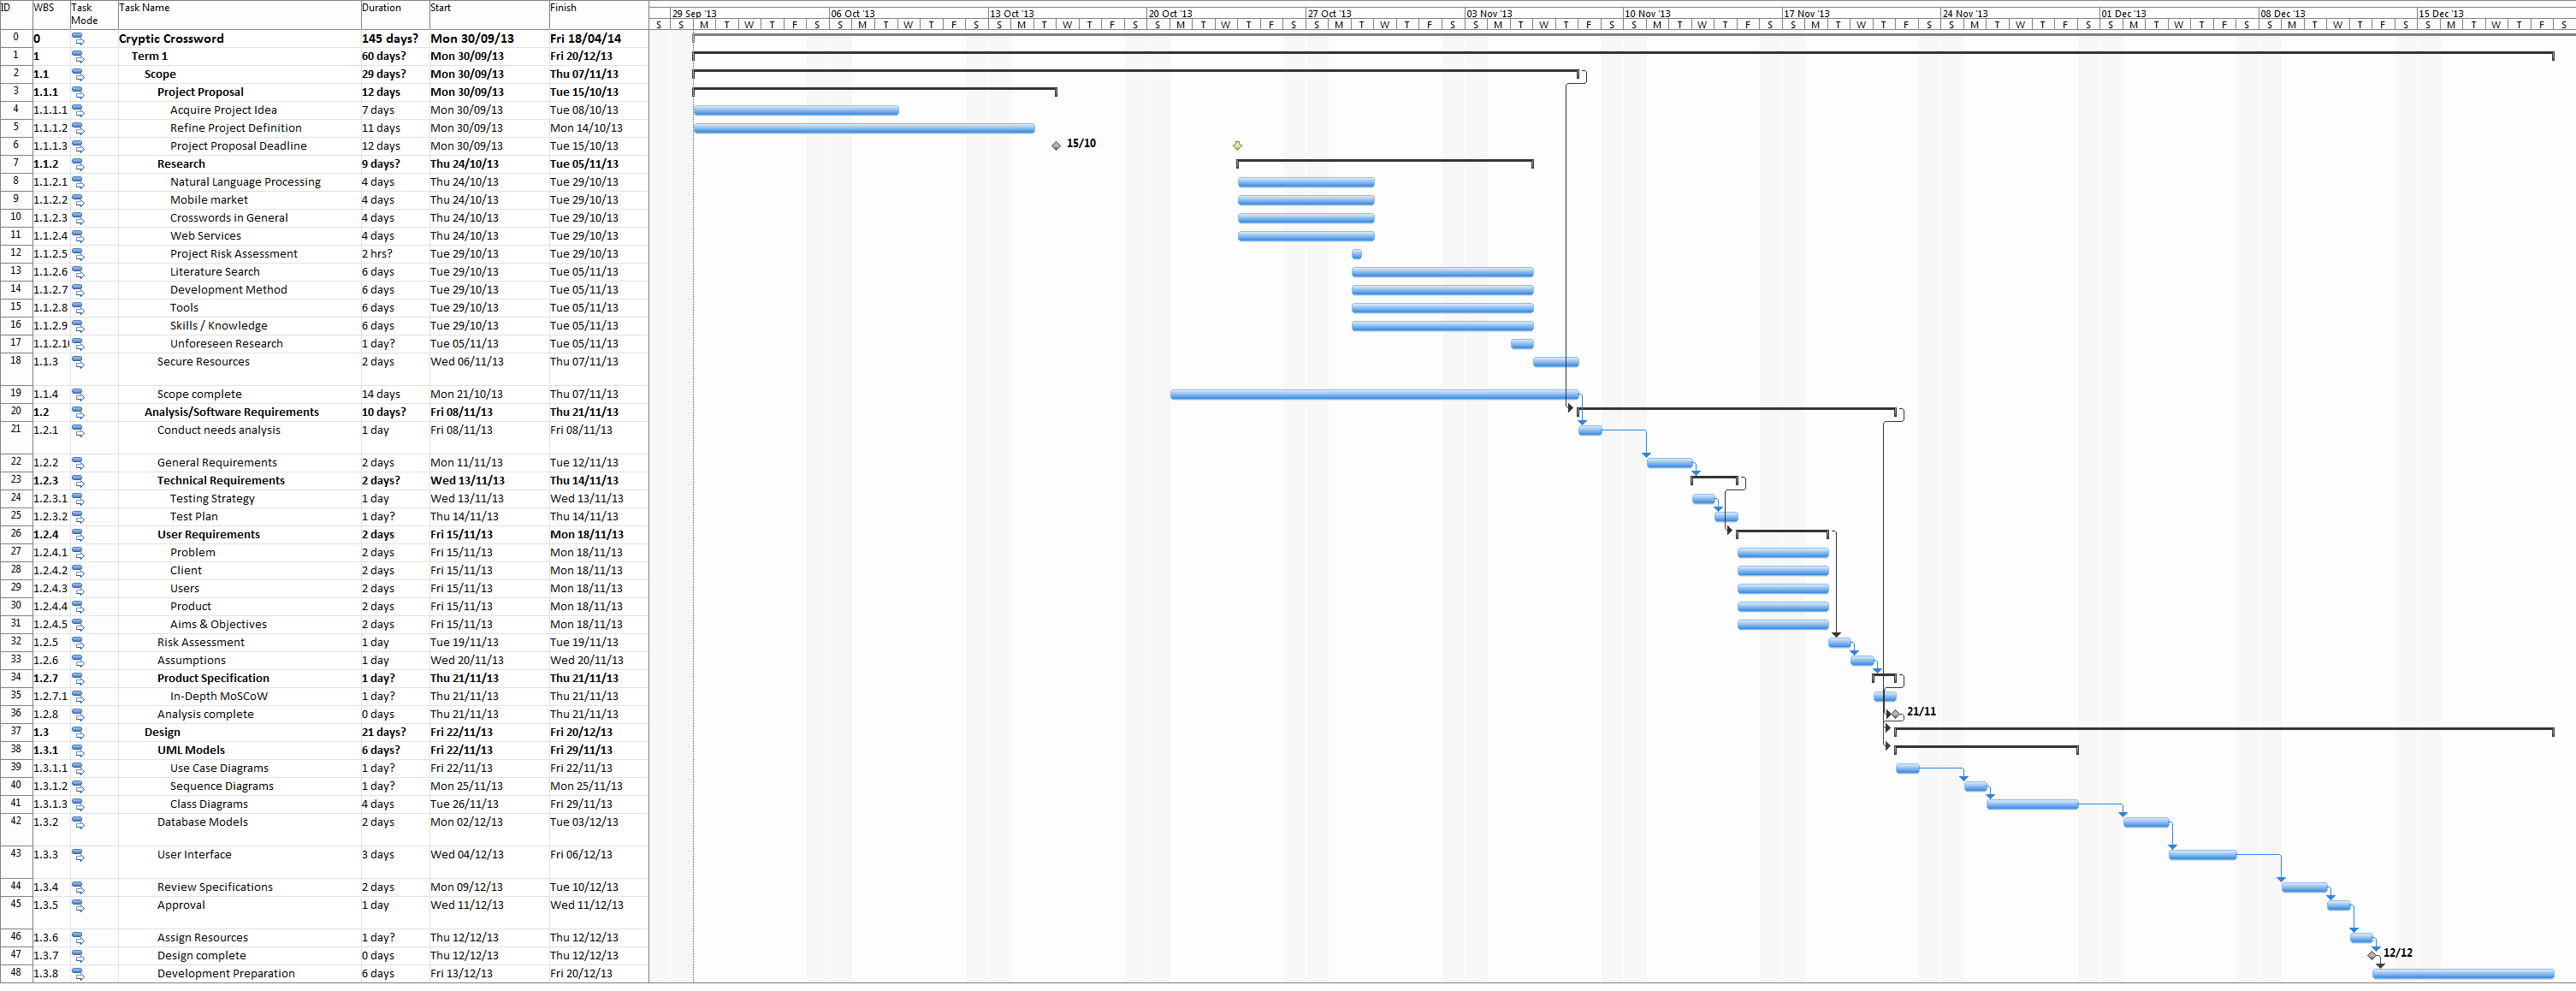
\includegraphics[width=\linewidth]{images/gant_chart1_term1.png}
  \caption{Gantt Chart for Term one produced on the 21st October 2013}
  \label{fig:gantt11}
\end{figure}

\begin{figure}[H]
  \centering
  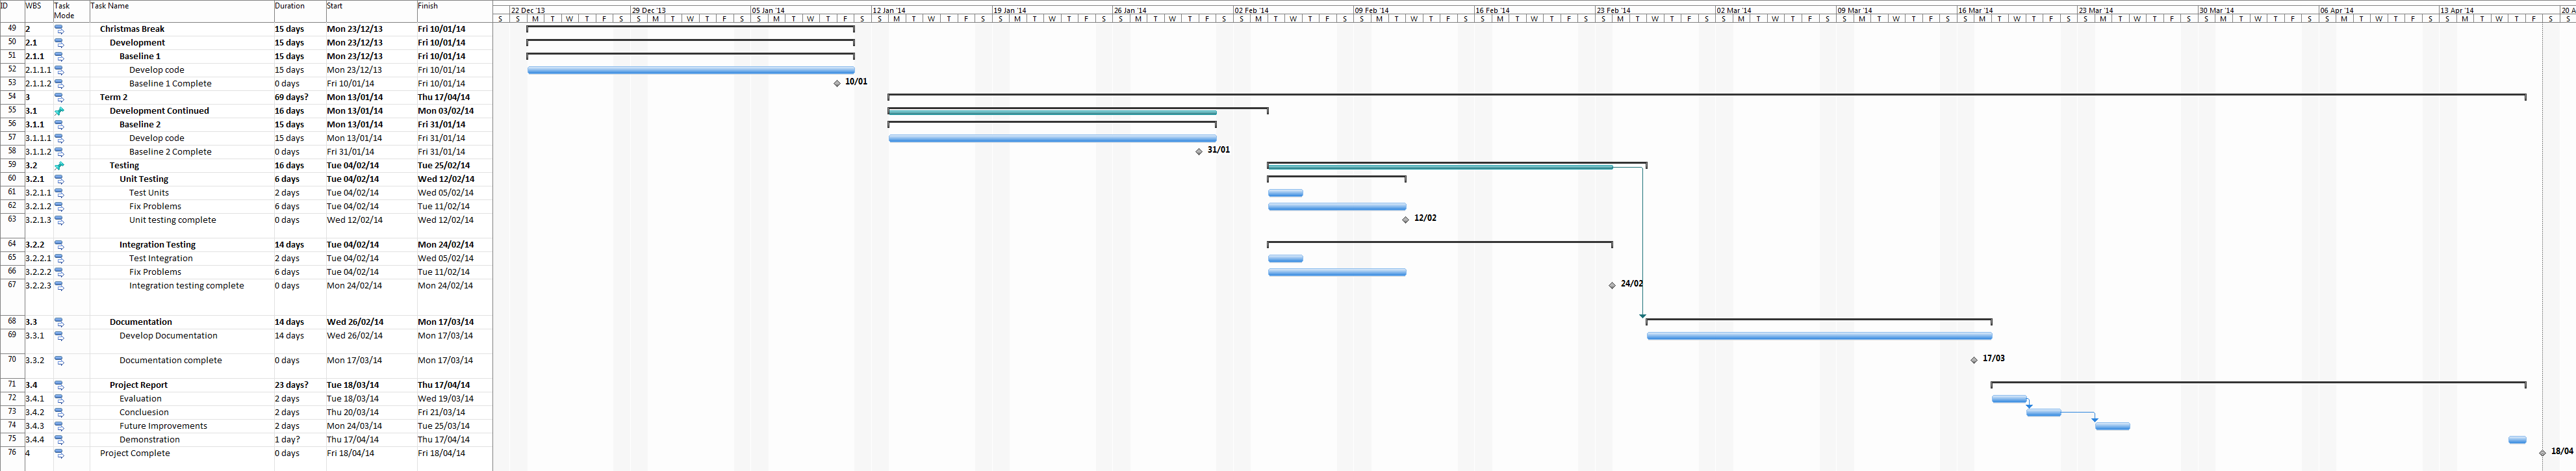
\includegraphics[width=\linewidth]{images/gant_chart1_term2.png}
  \caption{Gantt Chart for Term two produced on the 21st October 2013}
  \label{fig:gantt12}
\end{figure}


\newpage 
\subsection{Interim Gantt Chart}





\subsection{End Gantt Chart}

\end{landscape}
